Bij de system settings zitten zitten 3 tabs waaruit je kan kiezen:
\begin{itemize}
	\item Settings die betrekking op het motherboard, o.a. de instelling voor de hoeveelheid RAM van de VM.
	\item Settings die betrekking hebben op de CPU
	\item Settings die betrekking hebben op paravirtualisatie en het nesten van hardware virtualisatie (Acceleration)
\end{itemize}

De belangrijkste instelling bij Motherboard is vermoedelijk de toewijzing van de hoeveelheid RAM aan de VM. Andere opties zijn zaken die je bij een hardware systeem vaak in de BIOS tegen komt zoals de boot order en de tijd zoals deze doorgeven wordt aan het OS. Figuur \ref{VB_settings_system_mb} bevat ook nog andere opties die je kan instellen.
\begin{figure}[H]
	\centering
	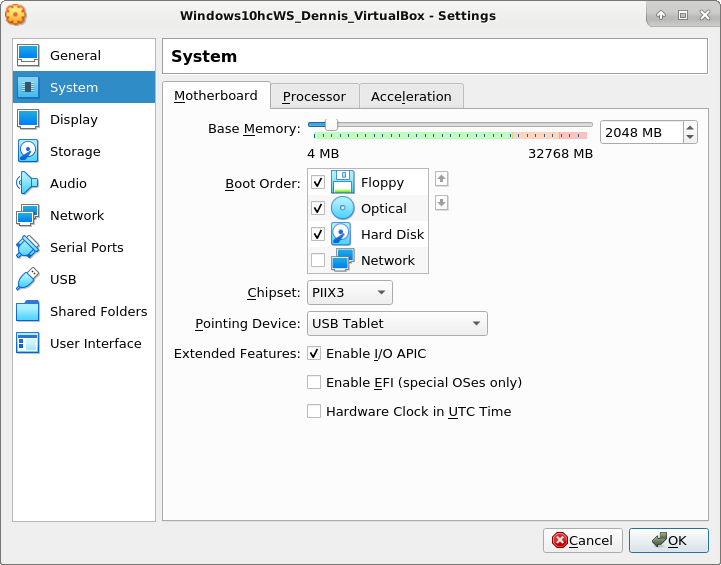
\includegraphics{virtualbox_vm_settings_motherboard.png}
	\caption{VirtualBox New VM}
	\label{VB_settings_system_mb}
\end{figure}

In de tab met Processor (\ref{VB_settings_system_cpu}) kan je aantal cores opgeven dat de VM mag gebruiken en kan je ook opgeven of de hardware virtualisatie doorgeven moet worden aan de VM zodat er nog een hypervisor op de VM ge\"installeerd kan worden.
\begin{figure}[H]
	\centering
	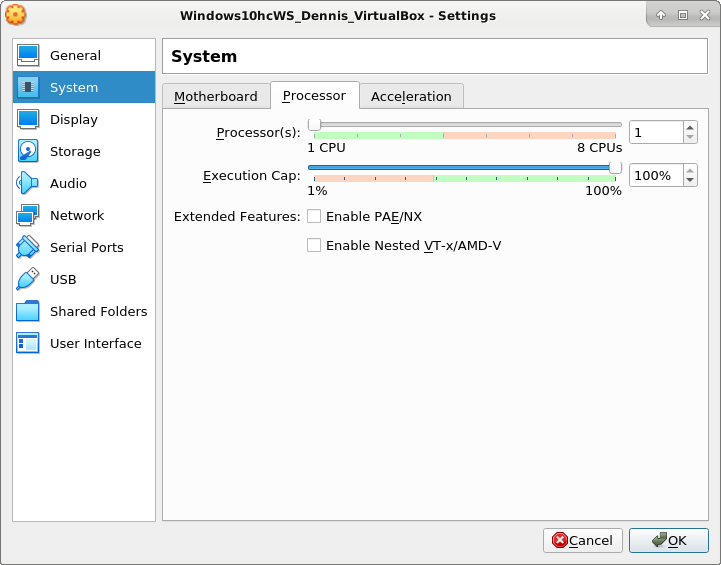
\includegraphics{virtualbox_vm_settings_processor.png}
	\caption{VirtualBox New VM}
	\label{VB_settings_system_cpu}
\end{figure}


\begin{figure}[H]
	\centering
	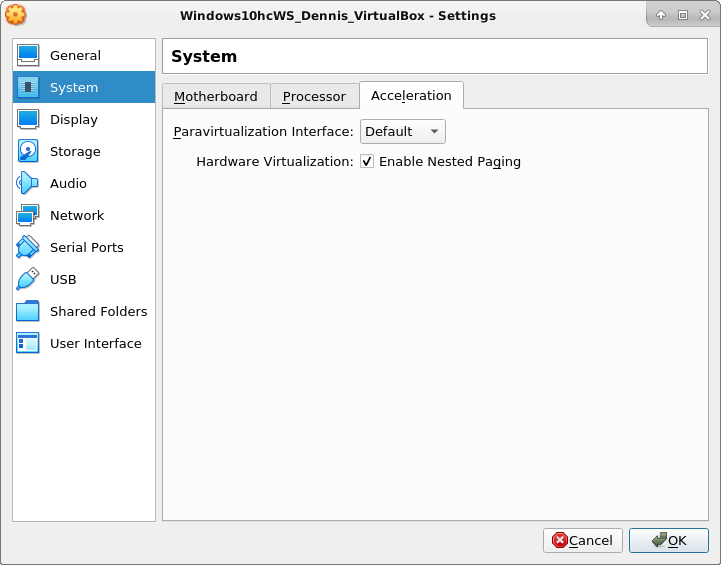
\includegraphics{virtualbox_vm_settings_acceleration.png}
	\caption{VirtualBox New VM}
	\label{VB_New_VM}
\end{figure}

